\documentclass[11pt]{article}
\usepackage[margin=1in]{geometry}
\usepackage{amsmath,amssymb,amsthm}
\usepackage{mathtools}
\usepackage{microtype}
\usepackage{graphicx}
\usepackage{booktabs}
\usepackage{xcolor}
\usepackage[hidelinks]{hyperref}

\graphicspath{{../figures/}}

\newtheorem{proposition}{Proposition}
\newtheorem{corollary}{Corollary}
\theoremstyle{remark}
\newtheorem{remark}{Remark}

\newcommand{\Bone}{B_1^{+}}
\newcommand{\Tone}{T_1}
\newcommand{\Ttwo}{T_2}
\newcommand{\Ttwos}{T_2^{*}}
\newcommand{\Rtwop}{R_2'}
\newcommand{\Mzero}{M_0}
\newcommand{\TR}{T_R}
\newcommand{\dw}{\Delta\omega}
\newcommand{\E}{\mathrm{e}}
\newcommand{\Fi}{\mathcal{I}}
\renewcommand{\Re}{\operatorname{Re}}

\title{Simultaneous $\Bone$ and $\Tone$ estimation in multi-pathway multi-echo (MPME)
imaging:\\ forward model and fundamental limits}
\author{Sarang Joshi}
\date{\today}

\begin{document}
\maketitle

\begin{abstract}
We derive the steady-state signal model of the multi-pathway multi-echo (MPME) sequence of
Cheng et al.~\cite{cheng2019} and analyse the joint estimation of the transmit field $\Bone$
and the longitudinal relaxation time $\Tone$ through the Fisher information and the
Cram\'er--Rao lower bound (CRLB). The central difficulty is a property of the
\emph{forward model}: for small flip angles and $\TR\ll\Tone$ every pathway amplitude is
invariant, to leading order, under $(\Mzero,\Bone,\Tone)\mapsto(\Mzero/\kappa,\,\kappa\Bone,\,\Tone/\kappa^2)$.
Protocols whose flip angles are all small therefore have a severely ill-conditioned
information matrix: the parameters remain identifiable in principle, but separating them
is extremely noise-sensitive (log-$\Tone$ bound of order one at realistic SNR). The
near-$360^\circ$ second pulse of the published protocol lifts the invariance through the
$2\pi$ wrap of the rotation, reducing the condition number from $5\times10^5$ to $173$. What
remains is a finite bound ($40.5\,\sigma/\Mzero$ on the standard deviation of $\log\Tone$)
set by the data. The published \emph{analytic inverse} adds an estimator-specific loss: in
Monte Carlo its $\Tone$ standard deviation is $3.2$--$7.1$ times the bound, with large bias
and undefined estimates at moderate SNR. A joint maximum-likelihood fit of the same model,
with the physical constraint $\Rtwop\ge0$ enforced, attains the bound (ratio $0.99$--$1.02$) at
the SNRs where its assumptions hold, and comes close at lower SNR where the constraint is
often active.
\end{abstract}

\section*{How to read this note}

Section~\ref{sec:model} builds the forward model from the configuration-state
(extended phase graph) description up to the measured voxel signal.
Section~\ref{sec:crlb} sets up the estimation-theoretic tools.
Section~\ref{sec:symmetry} proves the scaling invariance that underlies the $\Bone$/$\Tone$
problem and explains how the published protocol escapes it. Section~\ref{sec:results}
gives the bounds and the conditioning of the information matrix. Section~\ref{sec:inverse}
answers the question \emph{is the limitation in the forward model or in the inverse?} by
comparing the analytic reconstruction and a maximum-likelihood fit against the bound.
Table~\ref{tab:verdict} summarises the answer.

All numbers are reproducible with the code in the accompanying repository
(Appendix~\ref{app:repro}).

%=====================================================================================
\section{Forward model}\label{sec:model}
%=====================================================================================

\subsection{Sequence}

The MPME sequence is a 3D gradient-echo sequence without RF spoiling, with a constant RF
phase $\varphi$ and repetition time $\TR$. Only the readout gradient $G_x$ is unbalanced;
its net area per repetition, $A=\int_0^{\TR}G_x\,dt$, dephases the magnetisation by many
cycles across a voxel (the \emph{fully dephased} regime). Two acquisitions $i=1,2$ use the
same gradient waveform with nominal flip angles $\alpha_1^{\rm nom}=15^\circ$ and
$\alpha_2^{\rm nom}=330^\circ$ and $\TR=25$\,ms~\cite{cheng2019}. The actual flip angles are
\begin{equation}
  \alpha_i = \Bone\,\alpha_i^{\rm nom},
  \label{eq:b1}
\end{equation}
so $\Bone$ scales all pulses by the same factor.

Each of three readout windows of alternating polarity sweeps the cumulative gradient
moment through three adjacent integer multiples of $A$ (lobe areas
$+1.5:-3:+3:-3:+0.5$ in units of $-A$), sampling three \emph{pathways} (a two-pathway predecessor is described in~\cite{cheng2016})
$k\in\{+1,0,-1\}$ spaced by $1/\mathrm{BW}\approx 2$\,ms. A state of order $k$ created by
an RF pulse is refocused when the moment accumulated since the pulse equals $-kA$. This gives
each pathway three echo times $t_{ijk}\in(0,\TR)$ (in ms, assuming 4.5\,ms from the pulse to
the first echo): $k=+1$: $4.5,14.5,16.5$; $k=0$: $6.5,12.5,18.5$; $k=-1$: $8.5,10.5,20.5$.

\subsection{Configuration states}

Let $M^+=M_x+iM_y$ and let $\psi\in[0,2\pi)$ be the intravoxel phase imparted by one
repetition of the unbalanced gradient. Expand
\begin{equation}
  M^+(\psi)=\sum_{k}F_k\,\E^{ik\psi},\qquad M_z(\psi)=\sum_k Z_k\,\E^{ik\psi},\qquad
  Z_{-k}=\overline{Z_k}.
\end{equation}
One repetition of the operators acts as follows~\cite{weigel2015,hennig1991}.

\paragraph{RF pulse} (flip $\alpha$, phase $\varphi$; rotation
$R=R_z(\varphi)R_x(\alpha)R_z(-\varphi)$):
\begin{align}
  F_k' &= \cos^2\tfrac{\alpha}{2}\,F_k + \E^{2i\varphi}\sin^2\tfrac{\alpha}{2}\,\overline{F_{-k}}
          - i\E^{i\varphi}\sin\alpha\,Z_k,\\
  Z_k' &= -\tfrac{i}{2}\E^{-i\varphi}\sin\alpha\,F_k + \tfrac{i}{2}\E^{i\varphi}\sin\alpha\,
          \overline{F_{-k}} + \cos\alpha\,Z_k .
\end{align}
\paragraph{Relaxation} over $\TR$, with $E_1=\E^{-\TR/\Tone}$ and $E_2=\E^{-\TR/\Ttwo}$:
\begin{equation}
  F_k\to E_2F_k,\qquad Z_k\to E_1Z_k\ (k\neq0),\qquad Z_0\to E_1Z_0+\Mzero(1-E_1).
\end{equation}
\paragraph{Gradient} $F_k\to F_{k+1}$. Free precession by $\dw$ for a time $t$ multiplies
$M^+$ by $\E^{i\dw t}$ (same sense as the gradient twist).

\subsection{Steady state}

Write $a_k(\alpha,\Tone,\Ttwo,\TR)$ for the steady-state amplitude of $F_k$ immediately after
the RF pulse, per unit $\Mzero$. It can be computed exactly without truncating the state
space: an isochromat with total precession $\beta=\psi+\dw\TR$ per repetition has the
post-pulse steady state
\begin{equation}
  \bigl(I-R\,R_z(\beta)\,\mathrm{diag}(E_2,E_2,E_1)\bigr)\,\mathbf{M}^+
     = (1-E_1)\,R\,\hat{\mathbf z},
  \label{eq:iso}
\end{equation}
and $F_k$ is the $k$-th Fourier coefficient of $M^+(\psi)$ over $\psi$.

\begin{proposition}[Off-resonance only adds phase]\label{prop:offres}
In the fully dephased regime,
\[
  a_k(\dw)=a_k(0)\,\E^{ik\dw\TR};
\]
in particular $|a_k|$ does not depend on $\dw$.
\end{proposition}
\begin{proof}
By \eqref{eq:iso} the steady state depends on $\psi$ and $\dw$ only through
$\beta=\psi+\dw\TR$, so $M^+_{\dw}(\psi)=M^+_0(\psi+\dw\TR)$. Shifting a periodic
function by $\theta$ multiplies its $k$-th Fourier coefficient by $\E^{ik\theta}$.
\end{proof}

For the two lowest pathways the steady-state magnitudes have closed forms (unbalanced
FISP and PSIF), which we verified against \eqref{eq:iso} to $10^{-6}$:
\begin{align}
  |a_0| &= \Bigl|\tan\tfrac{\alpha}{2}\Bigl[1-\frac{(E_1-\cos\alpha)(1-E_2^2)}{r}\Bigr]\Bigr|,
  \label{eq:fisp}\\
  |a_{-1}| &= \Bigl|\frac{\tan\frac{\alpha}{2}}{E_2}\Bigl[1-\frac{(1-E_1\cos\alpha)(1-E_2^2)}{r}\Bigr]\Bigr|,
  \nonumber\\
  r^2 &= p^2-q^2,\quad p = 1-E_1\cos\alpha-E_2^2(E_1-\cos\alpha),\quad q=E_2(1-E_1)(1+\cos\alpha).
  \nonumber
\end{align}
The PSIF expression in the literature is the echo amplitude at $t=\TR$, hence the factor
$1/E_2$ for the post-pulse state.

\subsection{Echo evolution and the voxel signal}

Pathway $k$ read at time $t$ after the pulse carries, for one isochromat, the off-resonance
phase $\dw(t+k\TR)$ (Proposition~\ref{prop:offres} plus precession since the pulse).
Averaging over a Lorentzian intravoxel frequency distribution of half-width $\Rtwop$,
$\langle\E^{i\delta\tau}\rangle=\E^{-\Rtwop|\tau|}$, gives the signal of scan $i$, echo $j$,
pathway $k$:
\begin{equation}
  \boxed{\;S_{ijk}=\Mzero\,a_k\bigl(\Bone\alpha_i^{\rm nom},\Tone,\Ttwo,\TR\bigr)\,
  \E^{-t_{ijk}/\Ttwo}\,\E^{-\Rtwop|t_{ijk}+k\TR|}\,
  \E^{i(\phi_0+\dw(t_{ijk}+k\TR))}\;}
  \label{eq:signal}
\end{equation}
with $\Ttwos=1/(1/\Ttwo+\Rtwop)$. For $k\ge0$ the magnitude decays at $\Ttwo^{-1}+\Rtwop$;
for $k<0$ and $t<|k|\TR$ at $\Ttwo^{-1}-\Rtwop$ (a spin echo forming at $t=|k|\TR$).

\begin{remark}[Relation to the published equations]
Eq.~1 of~\cite{cheng2019}, $S=F^+\E^{-(R_2\pm\Rtwop)\mathrm{TE}}$ ($+$ for $k\ge0$), has
the same echo-time dependence as \eqref{eq:signal}; its intercept is
$F^+_k=a_k\E^{-\Rtwop|k|\TR}$. The extra factor depends only on $|k|$, so every relation
between the $\pm k$ states used in~\cite{cheng2019} (their Eqs.~4--13), and the mixing
factor, are unchanged. We verified numerically that their Eqs.~7, 16 and 17 hold exactly on
the steady states of \eqref{eq:iso} (Eq.~16 read as $\Tone=\TR/\ln[(Xc-1)/(X-c)]$).
\end{remark}

\subsection{Imaging and noise}

Image formation $y_{ijkc}=\mathcal{M}_i\mathcal{F}(C_c\,S_{ijk})+n_{ijkc}$ (coil maps
$C_c$, Fourier transform $\mathcal F$, sampling $\mathcal M_i$; scan 2 covers only the central
$25\%\times25\%$ of $k_y$--$k_z$) is linear. For the voxel-wise analysis below we model
the coil-combined complex images as $S_{ijk}+n_{ijk}$ with independent circular Gaussian
noise of standard deviation $\sigma$ per real and imaginary part.

%=====================================================================================
\section{Estimation-theoretic framework}\label{sec:crlb}
%=====================================================================================

Collect the unknowns of one voxel as
\begin{equation}
  \theta=(\log\Mzero,\ \log\Bone,\ \log\Tone,\ \log\Ttwo,\ \log\Ttwos,\ \dw,\ \phi_0).
\end{equation}
For the complex Gaussian model the Fisher information is
\begin{equation}
  \Fi(\theta)=\frac{1}{\sigma^2}\sum_{i,j,k}\Re\!\left[
     \overline{\partial_\theta S_{ijk}}\,\partial_\theta S_{ijk}^{\mathsf T}\right],
  \qquad
  \operatorname{Cov}(\hat\theta)\succeq\Fi^{-1}
\end{equation}
for any unbiased estimator (more precisely, any estimator that is locally unbiased at
$\theta$). Biased estimators, including constrained, regularised and learned ones, are not
covered: they can have smaller variance and smaller mean-squared error, at the price of a
bias that the CRLB does not quantify (for those, a Bayesian bound such as the van Trees
inequality is the appropriate tool). Because positive parameters enter through their
logarithm, $\sqrt{(\Fi^{-1})_{ll}}$ bounds the standard deviation of $\log\hat\theta_l$, which
equals the relative standard deviation of $\hat\theta_l$ only to first order (Section~\ref{sec:log}).
With $\sigma$ expressed in units of $\Mzero$ every bound scales as
$\sigma/\Mzero=1/\mathrm{SNR}(\Mzero)$; we report bounds \emph{per unit $\sigma/\Mzero$}. The brightest MPME image has
$|S|\approx0.088\,\Mzero$, so the image SNR is about $0.088\,\mathrm{SNR}(\Mzero)$.

We use three diagnostics of conditioning:
\begin{itemize}
\item the \emph{normalised information} $\tilde\Fi=D^{-1/2}\Fi D^{-1/2}$, $D=\mathrm{diag}\,\Fi$,
  its condition number $\kappa(\tilde\Fi)$, and its smallest eigenvalue $\lambda$ with
  eigenvector $u$. The eigenvector lives in normalised coordinates; the corresponding
  direction in the original coordinates is $w\propto D^{-1/2}u$, the solution of the
  generalised eigenproblem $\Fi w=\lambda Dw$. Conversely, a near-null direction $v$ of
  $\Fi$ appears in normalised coordinates as $u\propto D^{1/2}v$;
\item the \emph{variance inflation} $(\Fi^{-1})_{ll}\,\Fi_{ll}\ge1$, the factor by which the
  bound on $\theta_l$ grows because the other parameters are unknown;
\item the \emph{fixed-parameter bias}: if $\theta_m$ is held at a wrong value $\theta_m+\delta$
  and the rest is fitted, the estimates move by
  $\delta\theta_r=-\Fi_{rr}^{-1}\Fi_{rm}\,\delta$ to first order.
\end{itemize}
Jacobians are obtained by automatic differentiation through \eqref{eq:iso}--\eqref{eq:signal}
and checked against finite differences.

\subsection{Why logarithmic parameters}\label{sec:log}

The five quantities $\Mzero,\Bone,\Tone,\Ttwo,\Ttwos$ are positive \emph{scale} parameters:
they carry units (or, for $\Bone$, multiply a quantity that does), are only meaningful
relative to other scales in the problem, and are naturally compared by ratios. Their
logarithms are the natural coordinates for five reasons, of different weight.

\paragraph{1. The model depends on them only through dimensionless ratios.} Rewrite
\eqref{eq:signal} as
\begin{equation}
  \frac{S_{ijk}}{\Mzero}=G\Bigl(\Bone\alpha_i^{\rm nom},\ \frac{\TR}{\Tone},\
  \frac{\TR}{\Ttwo},\ \frac{t_{ijk}}{\Ttwo},\ \Rtwop t_{ijk},\ \dw\, t_{ijk}\Bigr),
  \label{eq:dimless}
\end{equation}
since $E_1=\E^{-\TR/\Tone}$, $E_2=\E^{-\TR/\Ttwo}$ and the echo terms depend only on products
of rates and times. A change of units, or a common rescaling of all times, is an additive
shift in log coordinates and leaves $G$ unchanged. The derivatives with respect to the log
parameters are dimensionless \emph{elasticities}, comparable across parameters:
\begin{align}
  \frac{\partial S}{\partial\log\Mzero}&=S, &
  \frac{\partial S}{\partial\log\Bone}&=\alpha_i\frac{\partial S}{\partial\alpha_i},\\
  \frac{\partial S}{\partial\log\Tone}&=-\frac{\TR}{\Tone}\,\frac{\partial S}{\partial(\TR/\Tone)}, &
  \frac{\partial S}{\partial\log\Ttwo}&=\frac{t}{\Ttwo}\,S
     -\frac{\TR}{\Ttwo}\,\frac{\partial S}{\partial(\TR/\Ttwo)}\Big|_{\rm steady\ state}.
  \nonumber
\end{align}
(The $\Ttwo$ elasticity is written at fixed $\Rtwop$; with $\Ttwos$ held fixed instead, as in
$\theta$, $\Rtwop=1/\Ttwos-1/\Ttwo$ also changes and contributes a further dimensionless term
$-\frac{|t+k\TR|}{\Ttwo}\,S$ (since $\partial\Rtwop/\partial\log\Ttwo=1/\Ttwo$), again a ratio of
times.)
In linear coordinates the corresponding columns of the Jacobian differ by factors of order
$\Tone/\Bone\sim10^3$ simply because of units, which says nothing about information.

\paragraph{2. The central symmetry is a straight line.} The invariance \eqref{eq:sym} is the
action of the multiplicative group $\kappa>0$,
$(\Mzero,\Bone,\Tone)\mapsto(\kappa^{-1}\Mzero,\kappa\Bone,\kappa^{-2}\Tone)$. In log
coordinates it is a translation,
\begin{equation}
  (\log\Mzero,\log\Bone,\log\Tone)\mapsto(\log\Mzero,\log\Bone,\log\Tone)+\log\kappa\,(-1,+1,-2),
\end{equation}
so the near-null direction $v=(-1,1,-2,0,0,0,0)$ of Corollary~\ref{cor:singular} is the
\emph{same constant vector at every point} of parameter space, and the orbits are straight
lines. In linear coordinates the orbits are curves $\{(\Mzero/\kappa,\kappa\Bone,\Tone/\kappa^2)\}$
whose tangent $(-\Mzero,\Bone,-2\Tone)$ changes from voxel to voxel, and the degeneracy can
only be stated locally. The scaling-type structure of the problem is what makes log
coordinates the ones in which it looks simplest.

\paragraph{3. The bounds become relative errors.} With $D=\mathrm{diag}(\Mzero,\Bone,\Tone,
\Ttwo,\Ttwos,1,1)$, the Fisher information in linear coordinates is
$\Fi_{\rm lin}=D^{-1}\Fi D^{-1}$, hence
\begin{equation}
  \sqrt{(\Fi^{-1})_{ll}}=\frac{\sqrt{(\Fi_{\rm lin}^{-1})_{ll}}}{\theta^{\rm lin}_l},
\end{equation}
which is the local (first-order) coefficient of variation. Relative error is the quantity
of clinical interest (a 30\,ms error matters at $\Tone=300$\,ms, not at 3000\,ms) and is
comparable across parameters with different units. For estimates, the delta method gives
$\operatorname{Var}(\log\hat\theta)\approx\operatorname{Var}(\hat\theta)/\theta^2$, again only
to first order. For large spreads the two differ substantially: if $\log\hat\theta$ has
standard deviation $s$ and is Gaussian, the coefficient of variation of $\hat\theta$ is
$\sqrt{\E^{s^2}-1}$, which is $\approx s$ for $s\lesssim0.2$ but $9.1$ for $s=2.1$. We
therefore call large values \emph{log-parameter spreads} and read them as multiplicative
factors: a spread $s$ corresponds to a one-sigma interval $[\theta\E^{-s},\theta\E^{s}]$.

\paragraph{4. The likelihood is closer to quadratic for the relaxation times.} The CRLB and
the asymptotic normality of maximum likelihood are second-order statements; they become
accurate at lower SNR in coordinates where the log-likelihood is closer to quadratic over
the noise-induced spread. We measured the asymmetry of the noise-free cost
$\|s(\theta)-s(\theta_0)\|^2$ for equal steps up and down in each coordinate, holding the
others fixed (reference tissue; a ratio of 1 means symmetric):
\begin{center}
\small
\begin{tabular}{lcccc}
\toprule
 & \multicolumn{2}{c}{$\pm20\%$} & \multicolumn{2}{c}{$\pm40\%$}\\
\cmidrule(lr){2-3}\cmidrule(lr){4-5}
Parameter & linear & log & linear & log\\
\midrule
$\Tone$ & 0.58 & 0.87 & 0.32 & 0.75\\
$\Ttwo$ & 0.78 & 1.16 & 0.60 & 1.34\\
$\Bone$ & 8.2 & 8.3 & 1.85 & 1.82\\
$\Mzero$ & 1.00 & 1.49 & 1.00 & 2.23\\
\bottomrule
\end{tabular}
\end{center}
The log coordinates are clearly better for $\Tone$, which has the largest bound and hence
the largest excursions, and somewhat better for $\Ttwo$. For $\Bone$ the asymmetry comes
from the $360^\circ$ structure of scan 2 and is the same in both coordinates. For $\Mzero$
linear coordinates are exactly quadratic, because the signal is linear in $\Mzero$. So
argument 4 does not justify $\log\Mzero$; arguments 2 and 3 do. Consistently, estimates of
relaxation times are right-skewed in linear units (for example $\Tone=\TR/\ln(\cdot)$ in
Eq.~16 has a heavy right tail), and we analyse Monte Carlo errors on $\log\hat\theta$, reporting
standard deviation, bias, RMSE and a robust spread side by side (Section~\ref{sec:inverse}).

\paragraph{5. Optimisation.} Log coordinates make positivity automatic. A step of size
0.1 is a $10\%$ change whatever the magnitude of the parameter, and the Jacobian columns
have comparable norms, so the damped Gauss--Newton steps are well scaled from the first
iteration. Positivity is not the whole physical domain, however: see the ordering
constraint below.

\paragraph{What does not depend on the choice.} The change from linear to log coordinates
has a diagonal Jacobian $D$. Therefore the correlation matrix of $\Fi^{-1}$, the
normalised information $\tilde\Fi$ (and its eigenvalues and condition number), the
variance inflation factors, and every statement of the form ``parameter $l$ is (not)
determined'' are \emph{identical} in both parameterisations at a given point. The
conclusions of Sections~\ref{sec:symmetry}--\ref{sec:inverse} do not rest on this
choice. What the logarithm adds is a global picture (straight symmetry orbits), unit-free
and relative error measures, better-behaved statistics, and easier optimisation.

\paragraph{Which parameters are not logged.} $\dw$ is a signed frequency and $\phi_0$ a
periodic phase: neither is a scale parameter, and both enter \eqref{eq:signal} linearly in
the exponent, so they stay linear. For the reversible decay we use $\log\Ttwos$ rather than
$\log\Rtwop$: $\Rtwop$ can be arbitrarily close to zero (here $\Rtwop=1/60-1/70$\,ms$^{-1}$),
and a relative error on a near-zero rate is large and uninformative. In the same
coordinates the bound on $\log\Rtwop$ is 366 per unit $\sigma/\Mzero$, against 47 for
$\log\Ttwos$, for exactly the same information.

\paragraph{The ordering constraint.} The Lorentzian model requires
$\Rtwop=1/\Ttwos-1/\Ttwo\ge0$, i.e.\ $\Ttwos\le\Ttwo$. Independent $\log\Ttwo$ and $\log\Ttwos$
coordinates enforce positivity of each but not this ordering. The CRLB is computed at an
interior point ($\Rtwop>0$) and is unaffected, but an estimator must enforce the ordering
explicitly; our maximum-likelihood fit projects onto $\log\Ttwos\le\log\Ttwo$
(Section~\ref{sec:ml}) and reports how often the constraint is active. When it is active
the estimator is no longer (locally) unbiased and the comparison with the CRLB loses its
footing for those voxels.

%=====================================================================================
\section{The fundamental limitation: a scaling invariance}\label{sec:symmetry}
%=====================================================================================

\begin{proposition}[Small-angle scaling invariance]\label{prop:scaling}
Let $\rho=\TR/\Tone$, $\varphi=0$, and fix $\TR$, $\Ttwo$ (hence $E_2<1$) and a pathway order
$k$. In the joint limit $\alpha\to0$, $\rho\to0$ with $c=\alpha^2/(2\rho)$ held fixed,
\begin{equation}
  a_k(\alpha,\Tone)=\alpha\,f_k(c,E_2)+O(\alpha^3+\alpha\rho),
  \label{eq:leading}
\end{equation}
with $f_k$ given in \eqref{eq:fk} below. Consequently, for any \emph{fixed} $\kappa>0$,
\begin{equation}
  \Mzero\,a_k(\alpha,\Tone)-\tfrac{\Mzero}{\kappa}\,a_k\bigl(\kappa\alpha,\ \Tone/\kappa^2\bigr)
  =O(\alpha^3+\alpha\rho),
\end{equation}
i.e.\ the signal \eqref{eq:signal} of every scan with a small flip angle, in every pathway
and echo, is invariant to leading order under
\begin{equation}
  (\Mzero,\ \Bone,\ \Tone)\ \longmapsto\ (\Mzero/\kappa,\ \kappa\Bone,\ \Tone/\kappa^2).
  \label{eq:sym}
\end{equation}
The remainder is additive (safe where $f_k$ is small) and is not uniform in $\kappa$: the
limit is taken with $\kappa$ fixed.
\end{proposition}

\begin{proof}
Work with one isochromat, $\dw=0$, and write $m_\perp=m_x+im_y$ and $m_z$ for the state just
after the pulse. Free precession and relaxation give the pre-pulse state
$m_\perp^-=E_2\E^{i\psi}m_\perp$, $Z\equiv m_z^-=E_1m_z+(1-E_1)$. The pulse $R_x(\alpha)$ gives
\begin{equation}
  m_\perp=m_\perp^- -i\sin\alpha\,Z + i(\cos\alpha-1)\,\mathrm{Im}\,m_\perp^-,\qquad
  m_z=\sin\alpha\,\mathrm{Im}\,m_\perp^- +\cos\alpha\,Z .
\end{equation}
In the steady state $Z=O(1)$ and $m_\perp=O(\alpha)$, so the last term in $m_\perp$ is
$O(\alpha^3)$ and $\sin\alpha=\alpha+O(\alpha^3)$. Solving the transverse equation,
\begin{equation}
  m_\perp=\frac{-i\alpha Z}{1-E_2\E^{i\psi}}+O(\alpha^3).
  \label{eq:mperp}
\end{equation}
The denominator is bounded away from zero, $|1-E_2\E^{i\psi}|\ge1-E_2>0$, uniformly in $\psi$.
For the longitudinal equation use $E_1=1-\rho+O(\rho^2)$, so
$m_z=Z-\rho(1-Z)+O(\rho^2)$, and $\cos\alpha=1-\alpha^2/2+O(\alpha^4)$:
\begin{equation}
  \rho(1-Z)=-\alpha\,\mathrm{Im}\,m_\perp^- +\tfrac{\alpha^2}{2}Z+O(\alpha^4+\rho^2+\alpha^2\rho).
\end{equation}
From \eqref{eq:mperp},
$\mathrm{Im}\,m_\perp^-=-\alpha Z\,\mathrm{Re}\bigl[E_2\E^{i\psi}/(1-E_2\E^{i\psi})\bigr]
=-\alpha Z\,(E_2\cos\psi-E_2^2)/|1-E_2\E^{i\psi}|^2$, and
\[
  \frac{E_2\cos\psi-E_2^2}{|1-E_2\E^{i\psi}|^2}+\frac12=\frac{1}{2}H(\psi),\qquad
  H(\psi)=\frac{1-E_2^2}{|1-E_2\E^{i\psi}|^2}=\frac{1-E_2^2}{1-2E_2\cos\psi+E_2^2}.
\]
Hence $\rho(1-Z)=\tfrac{\alpha^2}{2}H(\psi)\,Z$ to leading order, i.e.
$Z=\bigl[1+c\,H(\psi)\bigr]^{-1}$ with $c=\alpha^2/(2\rho)$, and
\begin{equation}
  m_\perp(\psi)=\frac{-i\alpha}{(1-E_2\E^{i\psi})\,\bigl[1+c\,H(\psi)\bigr]}+O(\alpha^3+\alpha\rho),
\end{equation}
where $1+cH\ge1$ keeps the expression uniformly bounded, so the remainder is uniform in
$\psi$. The pathway amplitude is the Fourier coefficient
\begin{align}
  a_k&=\frac{1}{2\pi}\int_0^{2\pi}m_\perp(\psi)\,\E^{-ik\psi}\,d\psi
  =\alpha\,f_k(c,E_2)+O(\alpha^3+\alpha\rho),\nonumber\\
  f_k(c,E_2)&=\frac{1}{2\pi}\int_0^{2\pi}\frac{-i\,\E^{-ik\psi}\,d\psi}{(1-E_2\E^{i\psi})[1+cH(\psi)]},
  \label{eq:fk}
\end{align}
and a uniform remainder in $\psi$ bounds the remainder of every Fourier coefficient. Under
$\alpha\to\kappa\alpha$, $\rho\to\kappa^2\rho$, $c$ is unchanged and the leading term scales
by $\kappa$, which $\Mzero\to\Mzero/\kappa$ compensates. Since $\Bone$ multiplies every flip
angle \eqref{eq:b1}, $\alpha\to\kappa\alpha$ is $\Bone\to\kappa\Bone$. The echo factors in
\eqref{eq:signal} do not involve $\alpha$ or $\Tone$.
\end{proof}

\begin{remark}[Checks]
For $k=0$ and $k=-1$ the same conclusion follows directly from the closed forms
\eqref{eq:fisp}: to leading order $E_1-\cos\alpha\simeq\alpha^2/2-\rho$,
$1-E_1\cos\alpha\simeq\rho+\alpha^2/2$ and $q\simeq2E_2\rho$ are homogeneous of degree one in
$(\rho,\alpha^2)$, so the brackets depend only on $c$, and $\tan(\alpha/2)\simeq\alpha/2$.
Numerically, with $c=0.75$, the leading-order formula \eqref{eq:fk} matches the exact solver
\eqref{eq:iso} for all pathways $k=-3,\dots,2$ with maximum error (relative to $|a_0|$)
$2.5\times10^{-3}$, $6.2\times10^{-4}$, $1.5\times10^{-4}$ and $3.8\times10^{-5}$ at
$\alpha=15^\circ,7.5^\circ,3.75^\circ,1.875^\circ$, the factor of four per halving expected from an
$O(\alpha^2)$ relative remainder; the scaling defect for $\kappa=2$ falls at the same rate.
On the full model with all three pathways and the $15^\circ/30^\circ$ protocol, fixing $\Bone$
wrong by $\varepsilon$ shifts the best fit by $\delta\log\Tone=-2.06\,\varepsilon$ and
$\delta\log\Mzero=-1.02\,\varepsilon$, against the predicted $-2$ and $-1$.
\end{remark}

\begin{corollary}[Leading-order degeneracy]\label{cor:singular}
Let $v=(-1,+1,-2,0,0,0,0)$ in the coordinates of $\theta$. If all flip angles are small,
$\partial_vS_{ijk}$ vanishes at leading order (it is $O(\alpha^3+\alpha\rho)$ while the other
directional derivatives are $O(\alpha)$), so $v^{\mathsf T}\Fi v$ is small relative to the
diagonal of $\Fi$ and $\Fi$ is ill-conditioned. Small-angle acquisitions, however many and
however their angles differ, cannot remove this leading-order degeneracy, because $\Bone$
scales all of them by the same factor.
\end{corollary}

\begin{remark}[What the corollary does and does not say]
The degeneracy is only of leading order. At finite angles the higher-order terms break it,
$\Fi$ is nonsingular, and the parameters are identifiable in principle; the corollary says
that separating them is extremely noise-sensitive. For the reference tissue the condition
number of $\tilde\Fi$ is $2.6\times10^4$ for $30^\circ/60^\circ$, $5.0\times10^5$ for
$15^\circ/30^\circ$ and $2.5\times10^7$ for $3.75^\circ/7.5^\circ$. Repeating acquisitions adds
information in the usual way (all bounds shrink as $1/\sqrt{N}$), so a sufficiently high SNR
resolves the poorly determined direction; it does not improve the conditioning. The bounds
apply to unbiased estimators. A biased estimator (a prior, regularisation, or a learned
network) can report a smaller spread along $v$, but that reduction comes from the prior,
not from the data.
\end{remark}

\subsection{How the published protocol escapes}

\begin{proposition}[Periodicity]\label{prop:period}
$|a_k(\alpha)|$ is even and $2\pi$-periodic in $\alpha$, and $a_k(-\alpha)=-a_k(\alpha)$ for
all $k$ (a global sign). Hence two protocols whose \emph{actual} flip angles agree up to sign
and multiples of $2\pi$ in every scan carry identical Fisher information about every
parameter when $\Bone$ is known. In particular, at $\Bone=1$ the protocols
$15^\circ/330^\circ$ and $15^\circ/30^\circ$ are equivalent with $\Bone$ known.
\end{proposition}
\begin{proof}
$R_x(-\alpha)=R_z(\pi)R_x(\alpha)R_z(-\pi)$, i.e.\ RF phase $\varphi=\pi$. Since precession
and relaxation commute with $R_z$, the steady state for phase $\pi$ is $R_z(\pi)$ applied
to the one for phase $0$, which multiplies every $F_k$ by $-1$. Periodicity is that of
$R_x$. A known, scan-wide sign does not change $\Fi$, and with $\Bone$ known the actual angles
are fixed.
\end{proof}

The equivalence is a statement about actual angles, not nominal ones: $330^\circ\Bone$ and
$-30^\circ\Bone$ agree modulo $360^\circ$ only when $360^\circ\Bone\equiv0$, i.e.\ at $\Bone=1$
within the physical range. At $\Bone=1.1$, for example, the second angles are $363^\circ$ and
$33^\circ$, and the known-$\Bone$ $\Tone$ bounds are 29.6 and 29.0 per unit $\sigma/\Mzero$.
Near $\Bone=1$ the information about $\Tone$ given $\Bone$ is therefore nearly the same for both
protocols, and the value of the large pulse lies in the $\Bone$ derivative. The effective
angle of scan 2 is $\alpha_2^{\rm eff}=330^\circ\Bone-360^\circ$, so
\begin{equation}
  \frac{\partial\log|\alpha_2^{\rm eff}|}{\partial\log\Bone}
  =\frac{330\,\Bone}{330\,\Bone-360},
  \qquad\text{whereas}\qquad
  \frac{\partial\log\alpha_1}{\partial\log\Bone}=+1 .
  \label{eq:lever}
\end{equation}
At $\Bone=1$ the first ratio is $-11$; it is $-2.75$ at $\Bone=0.8$ and diverges as
$\alpha_2^{\rm eff}\to360^\circ$. The invariance \eqref{eq:sym} requires all angles to scale by the
same factor; under a $\Bone$ change the second angle moves much faster and in the opposite
direction, so the near-null direction $v$ is lifted. The near-$360^\circ$ pulse acts as a
built-in $\Bone$ measurement.

\begin{remark}[Global ambiguity]
Proposition~\ref{prop:period} also implies that magnitudes cannot distinguish
$\alpha_2^{\rm eff}=360^\circ\mp x$. The sign of the scan-2 FID relative to scan 1 resolves
this branch (as in~\cite{cheng2019}), except at $\alpha_2^{\rm eff}=360^\circ$ exactly,
where that signal vanishes. This is a global identifiability issue that a local bound
cannot see; locally, $\Bone$ is determined \emph{best} near $360^\circ$
(Fig.~\ref{fig:sweeps}).
\end{remark}

%=====================================================================================
\section{Cram\'er--Rao bounds and conditioning}\label{sec:results}
%=====================================================================================

Unless stated otherwise the tissue is the reference used for protocol optimisation
in~\cite{cheng2019}: $\Tone/\Ttwo/\Ttwos=1500/70/60$\,ms, $\Bone=1$.

\begin{table}[h]
\centering
\caption{CRLB per unit $\sigma/\Mzero$: bound on the standard deviation of $\log\Mzero$,
$\log\Bone$, $\log\Tone$, $\log\Ttwo$, $\log\Ttwos$; rad/ms for $\dw$. Multiply by
$\sigma/\Mzero$ for a given SNR; the result approximates a relative standard deviation only
when it is small (Section~\ref{sec:log}).}
\label{tab:crlb}
\small
\begin{tabular}{llcccccc}
\toprule
Protocol & Tissue ($\Tone/\Ttwo/\Ttwos$, ms) & $\Mzero$ & $\Bone$ & $\Tone$ & $\Ttwo$ & $\Ttwos$ & $\dw$\\
\midrule
$15^\circ/330^\circ$ & WM ($850/66/50$) & 12.5 & 2.21 & 27.3 & 16.0 & 27.2 & 0.30\\
$15^\circ/330^\circ$ & GM ($1350/90/60$) & 14.7 & 2.75 & 33.1 & 20.7 & 38.2 & 0.31\\
$15^\circ/330^\circ$ & reference ($1500/70/60$) & 19.0 & 2.91 & 40.5 & 23.1 & 47.3 & 0.37\\
$15^\circ/330^\circ$ & reference, $\Bone$ known & 16.1 & -- & 28.0 & 20.7 & 44.2 & 0.37\\
\midrule
$15^\circ/30^\circ$ & reference & 1050 & 1020 & 2110 & 23.1 & 47.3 & 0.37\\
$15^\circ/30^\circ$ & reference, $\Bone$ known & 16.1 & -- & 28.0 & 20.7 & 44.2 & 0.37\\
\bottomrule
\end{tabular}
\end{table}

Table~\ref{tab:crlb} shows the two effects at once. With $15^\circ/30^\circ$ the
$\Mzero$--$\Bone$--$\Tone$ block is essentially singular while $\Ttwo$, $\Ttwos$ and $\dw$ are
untouched; with $\Bone$ known the two protocols coincide (Proposition~\ref{prop:period}).

\begin{table}[h]
\centering
\caption{Conditioning of the information matrix (reference tissue).}
\label{tab:cond}
\small
\begin{tabular}{p{0.40\linewidth}p{0.24\linewidth}p{0.26\linewidth}}
\toprule
 & $15^\circ/330^\circ$ & $15^\circ/30^\circ$\\
\midrule
Eigenvalues of $\tilde\Fi$ & $0.024,\ 0.11,\ 0.22,\ 0.51,$ $0.52,\ 1.49,\ 4.13$ &
  $7.7{\times}10^{-6},\ 0.11,\ 0.29,$ $0.51,\ 0.76,\ 1.49,\ 3.84$\\
Condition number $\kappa(\tilde\Fi)$ & 173 & $5.0\times10^{5}$\\
Variance inflation $\Mzero/\Bone/\Tone$ & $16.7/4.6/26.6$ & $51\,000/7\,700/72\,000$\\
Correlations $(\Bone,\Tone)$, $(\Bone,\Mzero)$, $(\Tone,\Mzero)$ & $0.72,\ 0.53,\ 0.77$ &
  $-0.9999,\ -0.9999,$ $0.9999$\\
$\partial\log\Tone/\partial\log\Bone$, $\Bone$ fixed, all data & $+10.1$ & $-2.06$\\
$\partial\log\Tone/\partial\log\Bone$, $\Bone$ fixed, scan 1 only & $-2.02$ & $-2.02$\\
\bottomrule
\end{tabular}
\end{table}

\begin{figure}[t]
\centering
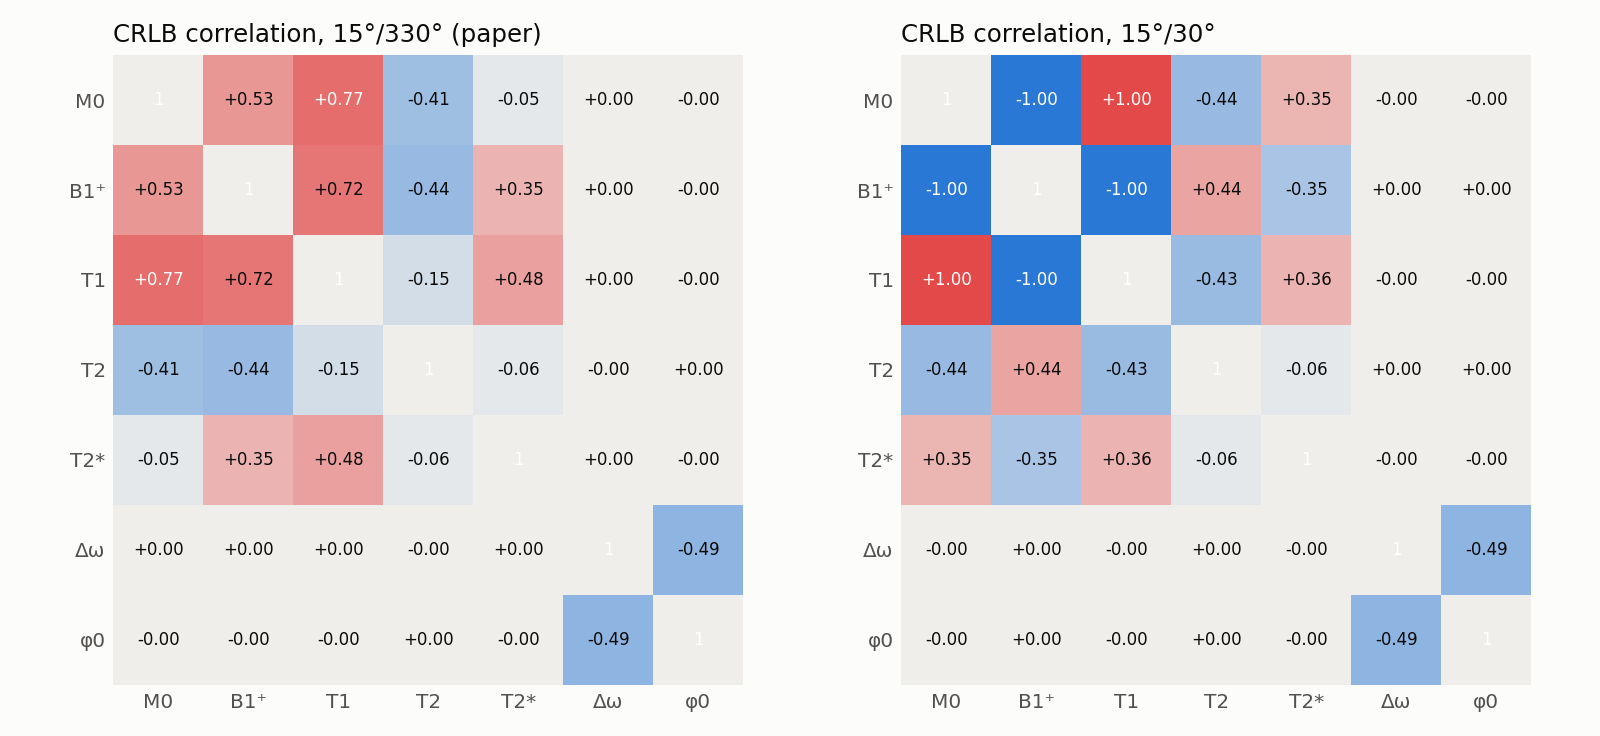
\includegraphics[width=\linewidth]{crlb_correlation.png}
\caption{Correlation matrices of the CRLB covariance $\Fi^{-1}$. Right: the
$\Mzero$--$\Bone$--$\Tone$ block of the small-angle protocol is perfectly correlated, the
signature of the invariance~\eqref{eq:sym}.}
\label{fig:corr}
\end{figure}

\begin{figure}[t]
\centering
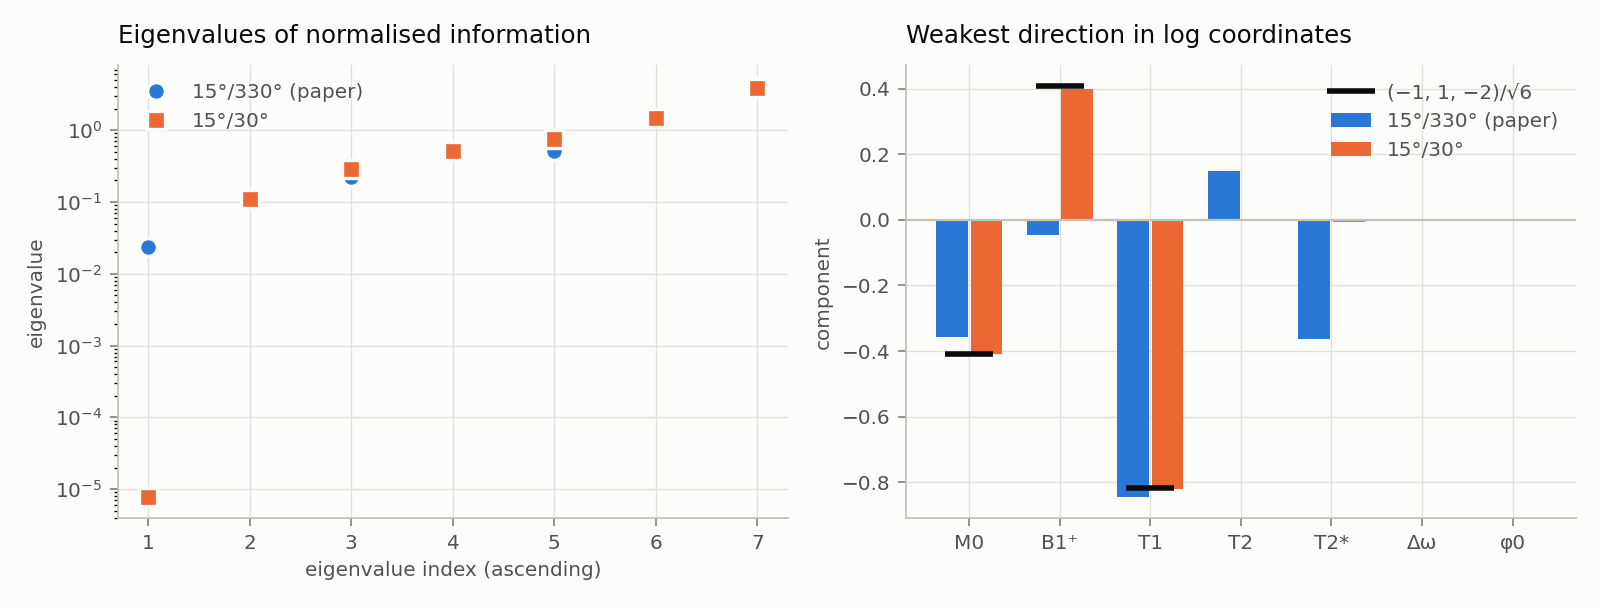
\includegraphics[width=\linewidth]{crlb_eigen.png}
\caption{Left: eigenvalues of the normalised information $\tilde\Fi$. Right: the weakest
direction mapped back to the original log coordinates, $w\propto D^{-1/2}u$ with $u$ the
eigenvector of the smallest eigenvalue of $\tilde\Fi$ (normalised to unit length, sign
fixed by the $\Tone$ component). For $15^\circ/30^\circ$ it coincides with the symmetry
direction $(-1,1,-2)/\sqrt6$ (black marks). For $15^\circ/330^\circ$ the smallest eigenvalue
is three thousand times larger and the weakest direction is mostly $\Tone$, with $\Mzero$ and
$\Ttwos$; its $\Bone$ component is only $-0.05$.}
\label{fig:eigen}
\end{figure}

\paragraph{Where the remaining $\Tone$ uncertainty comes from.} Freeing parameters one group
at a time gives the hierarchy
\begin{center}
\small
\begin{tabular}{lc}
\toprule
Unknown parameters & $\Tone$ bound (per unit $\sigma/\Mzero$)\\
\midrule
$\Tone$ only & 7.9\\
$+\ \Ttwo,\ \Ttwos,\ \dw,\ \phi_0$ & 21.1\\
$+\ \Mzero$ & 28.0\\
$+\ \Bone$ ($15^\circ/330^\circ$) & 40.5\\
$+\ \Bone$ ($15^\circ/30^\circ$) & 2110\\
\bottomrule
\end{tabular}
\end{center}
With the published protocol, freeing $\Bone$ last costs a factor 1.45; freeing the
transverse relaxation times costs 2.7 and $\Mzero$ 1.3. (These factors depend on the order
in which the groups are freed; the variance inflation factors of Table~\ref{tab:cond} are the
order-free summary.) At $15^\circ$ and $\TR=25$\,ms ($\Tone\gg\TR$), $\Tone$ is weakly encoded in
the steady-state amplitudes. Consistently, the weakest direction of the paper protocol in
log coordinates (Fig.~\ref{fig:eigen}) is dominated by $\Tone$ (component $-0.85$), with
$\Mzero$ and $\Ttwos$ ($-0.36$ each) and $\Ttwo$ ($+0.15$); its $\Bone$ component is only
$-0.05$. With this protocol $\Bone$ is no longer the main source of $\Tone$ uncertainty.

\paragraph{Which measurements carry the information.} Separating the data used from
whether $\Bone$ is known gives the $\Tone$ bounds
\begin{center}
\small
\begin{tabular}{lcc}
\toprule
Data & $\Bone$ unknown & $\Bone$ known\\
\midrule
both scans (full resolution) & 40.5 & 28.0\\
scan 1 only & $2.4\times10^{8}$ & 57.1\\
\bottomrule
\end{tabular}
\end{center}
Scan 1 alone cannot determine $\Bone$ and $\Tone$ jointly at all (a single small flip angle
is exactly the situation of Corollary~\ref{cor:singular}). With $\Bone$ known, adding the
high-flip scan still halves the bound on the standard deviation of $\log\Tone$ (57.1 to 28.0), because
scan 2 carries $\Tone$ information of its own.

\paragraph{Protocol dependence.} Fig.~\ref{fig:flip} shows that the $\Tone$ bound with
$\Bone$ unknown falls steeply with $\alpha_2^{\rm nom}$ and, from about $210^\circ$, stays
within $1.5\times$ of the $\Bone$-known bound. Over $(\alpha_1,\alpha_2)$ the optimum is
$10^\circ/340^\circ$ (bound 32.9), only $19\%$ better than $15^\circ/330^\circ$
(Fig.~\ref{fig:map}). Across a 3\,T-typical $\Bone$ range $0.7$--$1.3$ the $\Tone$ bound stays
between 40 and 65, and it grows with $\Tone$ itself (15 at 300\,ms, 100 at 4000\,ms;
Fig.~\ref{fig:sweeps}). Removing the $k=+1$ pathway raises the $\Tone$ bound from 40.5 to 67;
removing the echo pathway $k=-1$ raises it to 146 and the $\Ttwo$ bound from 23 to 208.

\begin{figure}[t]
\centering
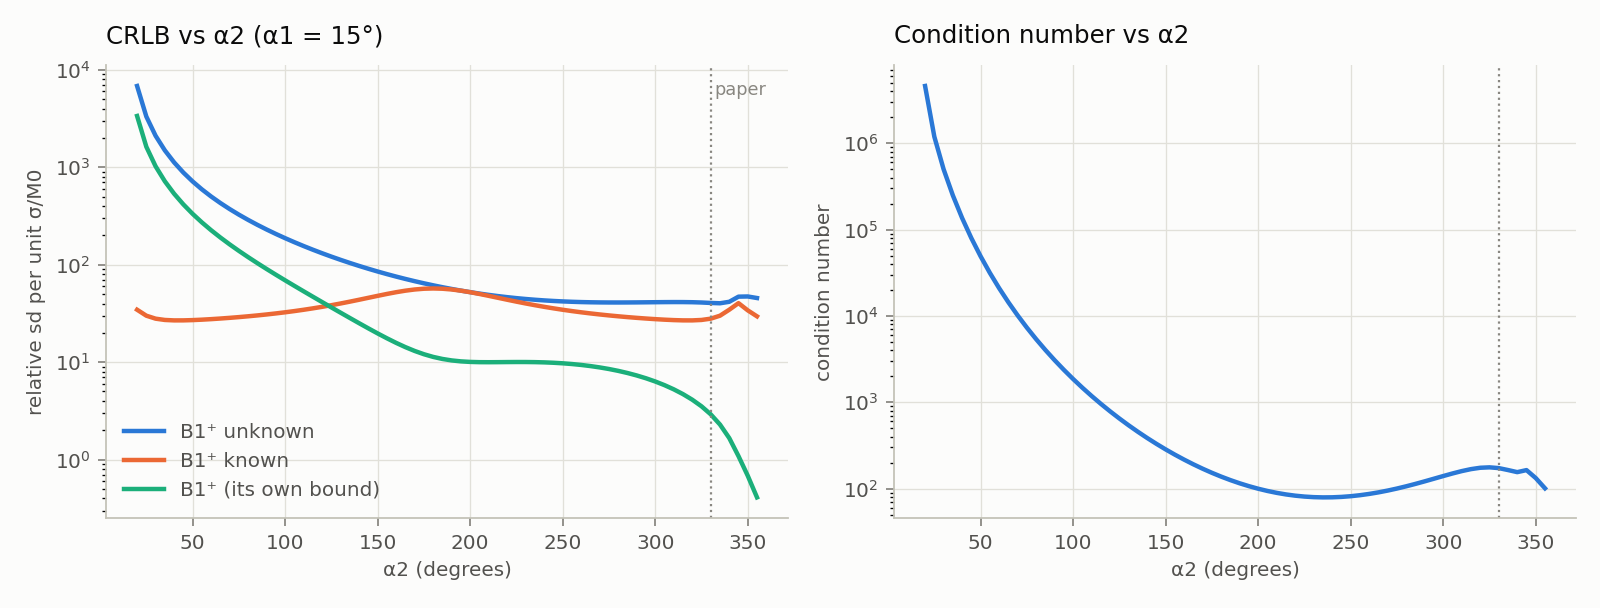
\includegraphics[width=\linewidth]{crlb_flip_sweep.png}
\caption{Bounds and condition number versus the nominal second flip angle
($\alpha_1^{\rm nom}=15^\circ$).}
\label{fig:flip}
\end{figure}

\begin{figure}[t]
\centering
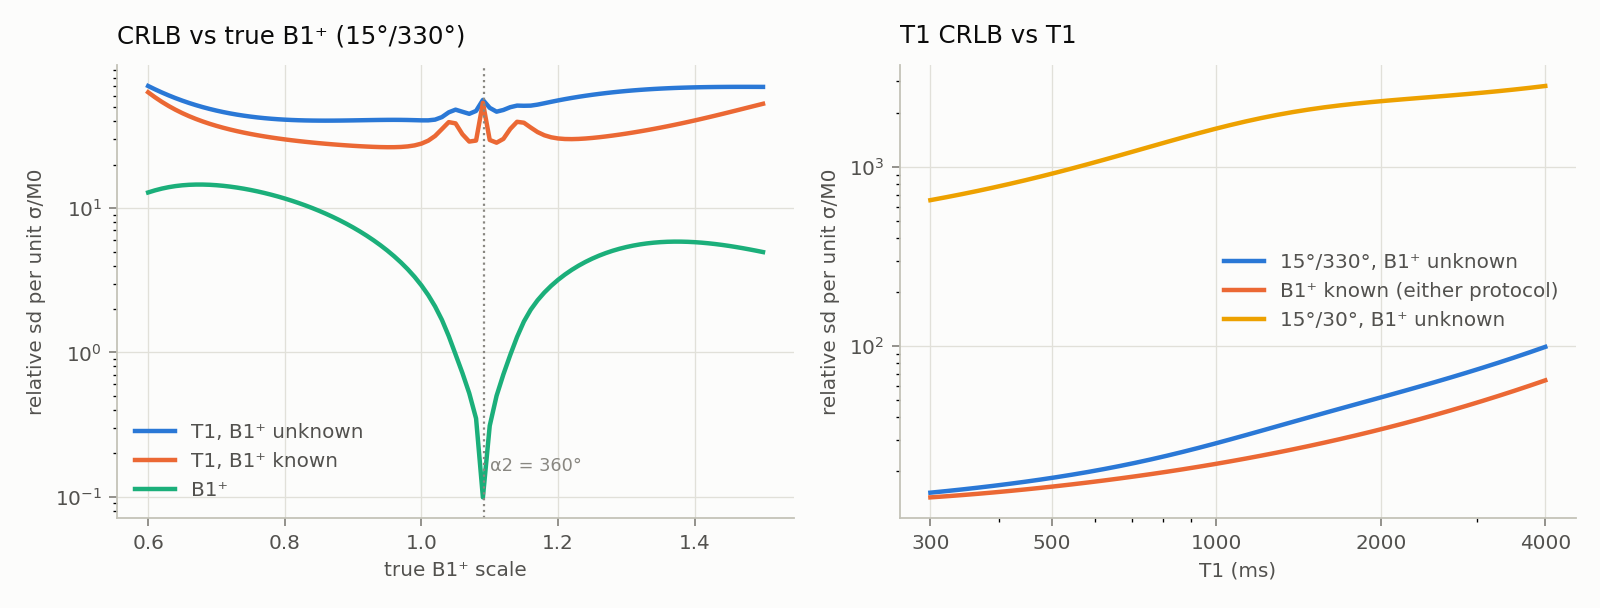
\includegraphics[width=\linewidth]{crlb_b1_t1_sweeps.png}
\caption{Left: bounds versus the true $\Bone$ for the published protocol; $\Bone$ is best
determined where $\alpha_2^{\rm eff}=360^\circ$. Right: $\Tone$ bound versus $\Tone$.}
\label{fig:sweeps}
\end{figure}

\begin{figure}[t]
\centering
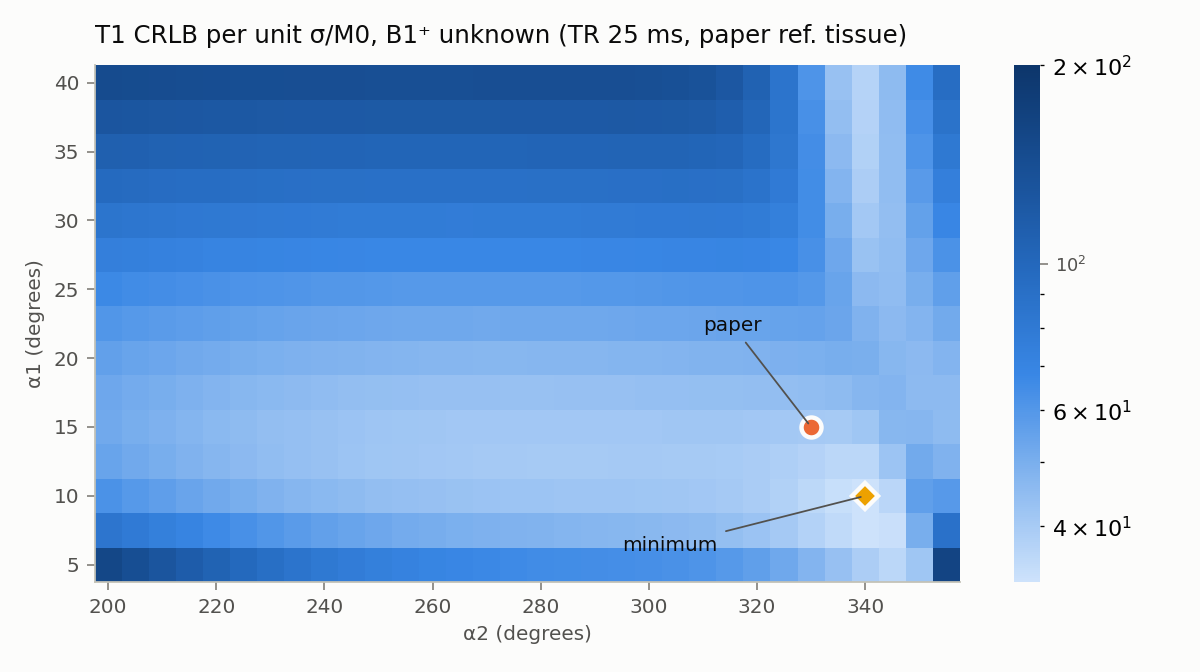
\includegraphics[width=0.8\linewidth]{crlb_flip_map.png}
\caption{$\Tone$ bound with $\Bone$ unknown over nominal $(\alpha_1,\alpha_2)$.}
\label{fig:map}
\end{figure}

%=====================================================================================
\section{Forward model or inverse?}\label{sec:inverse}
%=====================================================================================

The CRLB characterises the forward model and protocol; it says nothing about whether a
particular reconstruction attains it. To separate the two we compare three estimators of
the \emph{same} model on simulated data:
\begin{enumerate}
\item the \textbf{analytic inverse} of~\cite{cheng2019}, implemented equation by equation:
  $\dw$ from echo phases; $R_2$, $\Rtwop$ from a log-linear fit of their Eq.~1 to scan~1;
  real-valued $F$ states (Eq.~18); the mixing factor (Eqs.~10--11); the flip angle from
  Eq.~15; $\Tone$ and $\Mzero$ from Eqs.~16--17 using scan~1. We also run it with $\Bone$
  given, mimicking the paper's low-resolution, polynomial-smoothed $\Bone$ map;
\item a \textbf{model-fit baseline}: the same sequential structure, but with $\Bone$, $\Tone$,
  $\Mzero$ fitted by least squares to the FID and echo amplitudes of both scans;
\item a \textbf{joint maximum-likelihood (ML) fit} of \eqref{eq:signal} to all complex data
  (Section~\ref{sec:ml}).
\end{enumerate}
All three are exact on noise-free data (relative errors below $10^{-11}$ for the analytic
inverse). Table~\ref{tab:mc} reports robust standard deviations (interquartile range$/1.349$
of the log-estimates) over 1000 noise realisations.

\subsection{The joint maximum-likelihood estimator}\label{sec:ml}

\paragraph{Objective.} Stack the real and imaginary parts of all measured voxel signals
(2 scans $\times$ 3 pathways $\times$ 3 echoes) into $y\in\mathbb{R}^{36}$ and the model
\eqref{eq:signal} into $s(\theta)\in\mathbb{R}^{36}$, with $\theta$ as in
Section~\ref{sec:crlb}. Under independent Gaussian noise of variance $\sigma^2$ per
component the negative log-likelihood is, up to constants,
\begin{equation}
  -\log p(y\mid\theta)=\frac{1}{2\sigma^2}\,\|r(\theta)\|^2,\qquad r(\theta)=s(\theta)-y,
\end{equation}
so the ML estimate is the nonlinear least-squares solution
$\hat\theta=\arg\min_\theta\|r(\theta)\|^2$. It does not depend on $\sigma$. The model
$s(\theta)$ is evaluated with the exact steady-state solver \eqref{eq:iso} (256 isochromats),
so the estimator uses the same forward model as the CRLB, including all three pathways,
both scans, and the phase.

\paragraph{Parameterisation and constraints.} The five positive parameters are optimised
in log coordinates (Section~\ref{sec:log}); $\dw$ and $\phi_0$ are unconstrained. The fit is
a \emph{projected} Levenberg--Marquardt iteration: after every step the parameters are
projected onto
\begin{itemize}
\item the physical domain of the Lorentzian model, $\log\Ttwos\le\log\Ttwo$ ($\Rtwop\ge0$);
\item a safeguard box $\Bone\in[\E^{-1},\E]$, $\Tone\in[10,20\,000]$\,ms,
  $\Ttwo\in[1,5000]$\,ms, which excludes far-unphysical steps (at which the steady-state
  system can become singular).
\end{itemize}
For every voxel we record whether a constraint is active at the solution. Such estimates
are constrained ML estimates: they are not locally unbiased and are not covered by the
interior CRLB.

\paragraph{Initialisation.} The magnitude parameters and $\dw$ are taken from a sequential
estimator: the model-fit baseline, or the analytic inverse where its output is valid. The
global phase, which the sequential estimators do not provide, has a closed-form optimum
for fixed remaining parameters. With $S^{(0)}_{ijk}$ the model evaluated at the initial
values and $\phi_0=0$,
\begin{equation}
  \phi_0^{(0)}=\arg\Bigl(\sum_{i,j,k}S_{ijk}\,\overline{S^{(0)}_{ijk}}\Bigr),
\end{equation}
which minimises $\|r\|^2$ over $\phi_0$ alone.

\paragraph{Levenberg--Marquardt iteration.} Each voxel is fitted independently; all voxels
are processed in parallel as a batch. At iteration $n$, with
$J=\partial r/\partial\theta\in\mathbb{R}^{36\times7}$:
\begin{enumerate}
\item \emph{Jacobian.} Forward differences, $J_{:,l}=[r(\theta+h e_l)-r(\theta)]/h$ with
  $h=10^{-6}$ (all quantities in double precision).
\item \emph{Damped Gauss--Newton step} with Marquardt's diagonal scaling,
  \begin{equation}
    \bigl(J^{\mathsf T}J+\lambda\,\mathrm{diag}(J^{\mathsf T}J)\bigr)\,\Delta=-J^{\mathsf T}r,
    \qquad \theta_{\rm new}=\theta+\Delta .
  \end{equation}
  The diagonal scaling makes the step invariant to rescaling individual parameters, which
  matters here because the information matrix spans several orders of magnitude.
\item \emph{Acceptance.} If $\|r(\theta_{\rm new})\|^2<\|r(\theta)\|^2$ the step is accepted
  and $\lambda\leftarrow0.3\lambda$ (towards Gauss--Newton); otherwise it is rejected and
  $\lambda\leftarrow10\lambda$ (towards scaled gradient descent). $\lambda$ starts at
  $10^{-2}$ and is kept in $[10^{-9},10^{9}]$.
\end{enumerate}
We run a fixed 40 iterations. Near the optimum $\lambda\to0$ and the iteration becomes
Gauss--Newton. For a zero-residual problem (noise-free data) and a nonsingular Jacobian,
Gauss--Newton converges locally quadratically; in noise-free tests the parameters are
recovered to $10^{-15}$ relative error from starts perturbed by $5\%$. With noise the
residual at the solution is nonzero and the local convergence of Gauss--Newton is in general
only linear, with a rate governed by the residual size and the curvature of the model;
40 iterations were ample in our experiments (the cost no longer decreases).

\paragraph{Multiple starts.} Nonlinear least squares can converge to a local minimum, in
particular across the $360^\circ$ branch of the second flip angle or, for the small-angle
protocol, anywhere along the nearly flat symmetry valley \eqref{eq:sym}. We therefore run
the iteration from four starts and keep, per voxel, the solution with the lowest final
cost: the model-fit estimate; for $15^\circ/330^\circ$ the analytic-inverse estimate (where
valid), for $15^\circ/30^\circ$ the model-fit estimate moved along the symmetry direction
($\Bone\times1.1$, $\Tone/1.21$, $\Mzero/1.1$); and the model-fit estimate with $\Tone$ replaced by
700\,ms and by 2000\,ms (and $\Ttwos\le0.85\,\Ttwo$).

In simulation the global optimum can be checked: if the final cost exceeds the cost at the
true parameters, the optimiser has certainly not found the maximum likelihood. With only
the first two starts this happened in 19 of 1000 voxels at SNR$(\Mzero)=300$ (spurious
minima near $\Tone\approx6000$--$10\,000$\,ms with $\Rtwop=0$), which inflated the standard
deviation of $\log\hat\Tone$ from 0.13 to 0.26 and produced the heavy tails noted by a
reviewer of an earlier version. With four starts no voxel failed this check (Table~\ref{tab:mcdiag}).

\paragraph{When the ML fit should attain the bound.} At the solution, the Gauss--Newton
approximation of the covariance is $\sigma^2(J^{\mathsf T}J)^{-1}$, and
$J^{\mathsf T}J/\sigma^2$ evaluated at the true parameters is exactly the Fisher
information of Section~\ref{sec:crlb}. Under standard regularity conditions (interior true
parameter, identifiability, smoothness) the unconstrained ML estimator is consistent and
asymptotically efficient: as SNR$\to\infty$ its covariance converges to $\Fi^{-1}$ and its bias
vanishes. At finite SNR none of this is guaranteed. The estimator can be biased, it can
have heavy tails, and when constraints are active it can even have a variance \emph{below}
the bound, because it is then no longer unbiased. A meaningful efficiency comparison
therefore needs (i) the ordinary standard deviation, not only a robust spread, (ii) the
bias and RMSE, and (iii) the fraction of estimates on a constraint; Table~\ref{tab:mc}
reports all of them.

\paragraph{Cost.} Each iteration needs eight model evaluations (one plus seven
finite-difference directions). For $10^3$ voxels the full fit takes about a minute on a
laptop CPU. That is fast enough for simulation studies, but slow for whole-brain data
($\sim5\times10^6$ voxels), which is one motivation for the learned estimators in the
project plan.

\begin{table}[h]
\centering
\caption{Monte Carlo robust standard deviation (\%) of the log-estimates, 1000 noise realisations, reference tissue, $\Bone=1$. SNR is relative to $\Mzero$ (peak image SNR $\approx0.088\times$). Last column: fraction of voxels with undefined $\Tone$.}
\label{tab:mc}
\small
\begin{tabular}{lllccccc}
\toprule
Protocol & SNR$(\Mzero)$ & Estimator & $\Tone$ & $\Bone$ & $\Ttwo$ & $\Mzero$ & $\Tone$ undefined\\
\midrule
$15^\circ/330^\circ$ & 300 & CRLB & 13.5 & 1.0 & 7.7 & 6.3 & --\\
 &  & Joint ML & 13.7 & 0.9 & 7.5 & 6.0 & 0.0\%\\
 &  & Model fit & 90.7 & 3.7 & 36.8 & 56.9 & 0.0\%\\
 &  & Analytic inverse~\cite{cheng2019} & 102.6 & 46.1 & 37.0 & 57.1 & 1.9\%\\
 &  & Analytic inverse, $\Bone$ given & 35.9 & -- & -- & 23.3 & 1.9\%\\
\midrule
$15^\circ/330^\circ$ & 1000 & CRLB & 4.1 & 0.3 & 2.3 & 1.9 & --\\
 &  & Joint ML & 3.9 & 0.3 & 2.5 & 1.9 & 0.0\%\\
 &  & Model fit & 11.4 & 1.3 & 11.0 & 8.5 & 0.0\%\\
 &  & Analytic inverse~\cite{cheng2019} & 12.7 & 1.5 & 11.2 & 7.6 & 0.0\%\\
 &  & Analytic inverse, $\Bone$ given & 10.7 & -- & -- & 6.5 & 0.0\%\\
\midrule
$15^\circ/330^\circ$ & 3000 & CRLB & 1.4 & 0.1 & 0.8 & 0.6 & --\\
 &  & Joint ML & 1.3 & 0.1 & 0.8 & 0.6 & 0.0\%\\
 &  & Model fit & 4.0 & 0.4 & 3.8 & 2.9 & 0.0\%\\
 &  & Analytic inverse~\cite{cheng2019} & 4.4 & 0.4 & 3.7 & 2.6 & 0.0\%\\
 &  & Analytic inverse, $\Bone$ given & 3.9 & -- & -- & 2.2 & 0.0\%\\
\midrule
$15^\circ/30^\circ$ & 1000 & CRLB & 210.6 & 102.3 & 2.3 & 104.8 & --\\
 &  & Joint ML & 211.7 & 103.7 & 2.2 & 105.3 & 0.0\%\\
 &  & Model fit & 287.6 & 138.0 & 11.0 & 149.0 & 0.0\%\\
\midrule
$15^\circ/30^\circ$ & 3000 & CRLB & 70.2 & 34.1 & 0.8 & 34.9 & --\\
 &  & Joint ML & 77.1 & 37.3 & 0.7 & 38.1 & 0.0\%\\
 &  & Model fit & 225.6 & 109.7 & 3.8 & 113.9 & 0.0\%\\
\bottomrule
\end{tabular}
\end{table}


\paragraph{Reading Tables~\ref{tab:mc}--\ref{tab:mcdiag}.} All ratios below use ordinary
standard deviations (SD); robust spreads are listed alongside because they can hide heavy
tails. The Monte Carlo standard error of an SD estimated from 1000 samples is about $2\%$.
\begin{itemize}
\item \textbf{The bound is attained where its assumptions hold.} For $15^\circ/330^\circ$ at
  SNR$(\Mzero)=1000$ and $3000$ the joint ML fit has SD/CRLB between 0.99 and 1.02 for
  $\Tone$, $\Bone$, $\Ttwo$ and $\Mzero$, negligible bias ($|\text{mean}|<10^{-3}$ in log units),
  no constrained estimates (at most $0.3\%$) and no optimiser failures. In this regime the
  forward model \emph{contains} the information that Table~\ref{tab:crlb} promises, and an
  estimator extracts it; the published protocol can separate $\Bone$ and $\Tone$.
\item \textbf{At SNR 300 the comparison is only approximate.} The ML SD/CRLB is 1.00 for
  $\Bone$ and 0.95 for $\Tone$, but the constraint $\Rtwop\ge0$ is active in $19.5\%$ of voxels
  (true $\Rtwop$ is small: $\Ttwos=60$ vs $\Ttwo=70$\,ms). Those estimates are not unbiased, which
  is how the $\Tone$ SD can fall slightly below the bound. The bias is small
  ($-0.007$ in $\log\Tone$).
\item \textbf{The analytic inverse is well above the bound.} Its $\Tone$ SD is $3.2\times$ the
  bound at SNR 3000, $5.1\times$ at SNR 1000 and $7.1\times$ at SNR 300, where it is also
  strongly biased ($+0.44$ in $\log\Tone$, a factor $1.56$) and $1.9\%$ of voxels have no valid
  $\Tone$ (Eq.~16 needs $(Xc-1)/(X-c)>1$). Its $\Bone$ SD is $4.8\times$ the bound at SNR 3000 but
  $23\times$ and $28\times$ at SNR 1000 and 300, with heavy tails (SD much larger than the
  robust spread at SNR 1000). The model-fit baseline, which shares the sequential structure
  but not the closed forms, is similar ($\Tone$: $2.8\times$, $3.9\times$, $7.0\times$): the loss
  comes mainly from the sequential structure.
\item \textbf{With $\Bone$ given, compare with the matched bound.} The analytic inverse
  computes $\Tone$ from scan 1 with $\Bone$ fixed, so its matched bound is the scan-1,
  $\Bone$-known bound of 57.1 per unit $\sigma/\Mzero$. Its SD is then $1.9\times$ that bound at SNR
  1000 and 3000 and $2.8\times$ at SNR 300 (Table~\ref{tab:mcdiag}). Against the two-scan,
  $\Bone$-known bound of 28.0 the ratios are $3.8$--$5.7$; against the $\Bone$-unknown bound of
  40.5 (the reference used in an earlier version of this note) the comparison is not
  like-for-like.
\item \textbf{The small-angle control does not support an efficiency claim.} For
  $15^\circ/30^\circ$ the safeguard box is active in $35\%$ (SNR 1000) and $10\%$ (SNR 3000) of ML
  estimates, which are biased ($+0.41$ and $+0.24$ in $\log\Tone$). At SNR 1000 the ML SD is
  therefore \emph{below} the bound (0.65 of it), and at SNR 3000 above it (1.23); neither
  comparison is meaningful, because the estimator is bounded and biased. What the control
  does show is that the bound itself is of order one in log units: 2.1 in $\log\Tone$ at SNR
  1000, i.e.\ a one-sigma factor of $\E^{2.1}\approx8$, and still 0.70 (a factor 2) at SNR 3000,
  while $\Ttwo$ is unaffected. With small angles, $\Bone$ and $\Tone$ cannot be separated
  usefully at these SNRs by any unbiased estimator; this is the forward model and protocol
  (Corollary~\ref{cor:singular}).
\end{itemize}

\paragraph{Sources of the estimator-specific loss.} The analytic inverse (i) is
\emph{sequential}: $R_2$ and $\Rtwop$ are fixed from scan~1 before the flip angle and
$\Tone$ are estimated, so their errors propagate instead of being traded off jointly;
(ii) uses \emph{closed-form nonlinear transformations} (differences of extrapolated
states, ratios, logarithms) whose noise amplification is not controlled and whose domain
can be left by noise; (iii) computes $\Tone$ from \emph{scan~1} only, with $\Bone$ held
fixed; and (iv) discards phase (Eq.~18), which costs little here because $\dw$ and $\phi_0$
decouple from the other parameters (Fig.~\ref{fig:corr}).

Point (iii) combines two separate changes relative to the joint bound of 40.5, which the
table in Section~\ref{sec:results} separates: treating $\Bone$ as known (40.5 to 28.0 with
both scans) and dropping scan 2 from the $\Tone$ step (28.0 to 57.1 with $\Bone$ known). The
matched reference for the analytic inverse with $\Bone$ given is therefore 57.1, not 40.5 or
28.0 (Table~\ref{tab:mcdiag}). In addition, holding $\Bone$ fixed turns a $\Bone$ error
$\varepsilon$ into a $\Tone$ bias of $-2.02\,\varepsilon$ in this step (Table~\ref{tab:cond}).
Dropping scan 2 is partly an acquisition choice: scan~2 is acquired only at low resolution,
so a full-resolution bound using both scans is not available to any estimator in the
published design. At the low resolution both scans have about four times the per-voxel SNR,
giving a $\Bone$ bound of $2.91/4\approx0.73$ per low-resolution voxel before spatial
smoothing.

\begin{table}[h]
\centering
\caption{Origin of each difficulty.}
\label{tab:verdict}
\small
\begin{tabular}{p{0.38\linewidth}p{0.2\linewidth}p{0.34\linewidth}}
\toprule
Difficulty & Origin & Remedy\\
\midrule
Leading-order $\Mzero$--$\Bone$--$\Tone$ invariance \eqref{eq:sym} for small flip angles
  (severe ill-conditioning, not exact singularity) &
  forward model $+$ protocol & a pulse whose effective angle does not scale with $\Bone$
  (e.g.\ near $360^\circ$, as published); otherwise very high SNR\\
Residual $\Tone$ bound (40.5 per unit $\sigma/\Mzero$): confounding with $\Ttwo$, $\Ttwos$,
  $\Mzero$, $\Bone$ & forward model $+$ protocol & SNR, averaging, spatial priors; protocol
  tuning ($\le20\%$)\\
Branch ambiguity $360^\circ\mp x$ & forward model (periodicity) & phase of the scan-2 FID\\
Error well above the bound; large bias and undefined $\Tone$ at moderate SNR &
  analytic inverse (sequential, closed-form) & joint (ML or learned) estimation\\
$\Tone$ bound 57.1 instead of 28.0 with $\Bone$ known; $\Tone$ bias $-2\varepsilon$ per $\Bone$
  error $\varepsilon$ & design: scan-1-only $\Tone$ step, low-resolution scan~2 &
  joint estimation with a smooth-$\Bone$ prior\\
Constrained estimates ($\Rtwop=0$) at low SNR & forward model domain $+$ small true $\Rtwop$ &
  report; Bayesian or constrained bounds\\
In-vivo calibration $\beta=1.24$ (Eq.~19 of~\cite{cheng2019}) & model mismatch (not
  variance) & richer forward model (finite pulses, MT, \dots)\\
\bottomrule
\end{tabular}
\end{table}

%=====================================================================================
\section{Implications}
%=====================================================================================

\begin{enumerate}
\item The published protocol is sound from an information standpoint: the near-$360^\circ$
  pulse lifts the leading-order invariance that makes $\Bone$/$\Tone$ separation extremely
  noise-sensitive with small angles.
\item No \emph{unbiased} voxel-wise estimator can beat Table~\ref{tab:crlb}. The realistic
  voxel-wise gain of an unbiased estimator over the analytic inverse is the gap that the ML
  fit closes (Table~\ref{tab:mc}). Biased estimators, including learned ones trained with a
  prior over tissue parameters, can have lower variance or MSE than the bound; their benefit
  then comes from the prior, and their bias must be characterised (for example with a
  Bayesian bound) rather than ignored.
\item Larger gains require prior information across voxels. $\Bone$ is spatially smooth,
  so treating it as nearly known removes its factor 1.45; the remaining confounding with
  $\Mzero$ and the transverse relaxation times can only be reduced by image priors.
\item When $\Bone$ is supplied to a joint estimator that also uses the high-flip data, a
  $\Bone$ error is amplified about tenfold into $\Tone$ (Table~\ref{tab:cond}); $\Bone$ should
  be estimated jointly or the high-flip data excluded from the $\Tone$ step.
\end{enumerate}

\paragraph{Caveats.} The CRLB is local and assumes an exact model, Gaussian noise, an
interior true parameter and (locally) unbiased estimators; constrained or biased estimates
fall outside it. The model uses instantaneous RF pulses (no off-resonance nutation,
Eq.~8 of~\cite{cheng2019}), a Lorentzian $\Rtwop$ line shape, no diffusion and no
magnetisation transfer. The time from the pulse to the first echo is assumed. Except where
stated, both scans are treated at full resolution.

\appendix
\section{Reproducibility}\label{app:repro}

\begin{tabular}{ll}
Forward model & \texttt{src/mpme/epg.py}, \texttt{signal.py}, \texttt{sequence.py}\\
Analytic inverse of~\cite{cheng2019} & \texttt{src/mpme/paper.py}\\
Model-fit baseline & \texttt{src/mpme/analytic.py}\\
Joint ML fit & \texttt{src/mpme/mle.py}\\
Fisher information, CRLB & \texttt{src/mpme/crlb.py}\\
Tables~\ref{tab:crlb}--\ref{tab:cond}, figures & \texttt{python scripts/crlb\_analysis.py}\\
Table~\ref{tab:mc} & \texttt{python scripts/estimator\_efficiency.py}\\
\end{tabular}

\begin{thebibliography}{9}
\bibitem{cheng2019} C.-C.~Cheng, F.~Preiswerk, W.~S.~Hoge, T.-H.~Kuo, B.~Madore.
  Multipathway multi-echo (MPME) imaging: all main MR parameters mapped based on a single
  3D scan. \emph{Magn.\ Reson.\ Med.} 81(3):1699--1713, 2019.
\bibitem{cheng2016} C.-C.~Cheng, C.-S.~Mei, J.~Duryea, H.-W.~Chung, T.-C.~Chao,
  L.~P.~Panych, B.~Madore. Dual-pathway multi-echo sequence for simultaneous frequency and
  $T_2$ mapping. \emph{J.\ Magn.\ Reson.} 265:177--187, 2016.
\bibitem{hennig1991} J.~Hennig. Echoes---how to generate, recognize, use or avoid them in
  MR-imaging sequences. \emph{Concepts Magn.\ Reson.} 3(3):125--143, 1991.
\bibitem{weigel2015} M.~Weigel. Extended phase graphs: dephasing, RF pulses, and
  echoes---pure and simple. \emph{J.\ Magn.\ Reson.\ Imaging} 41(2):266--295, 2015.
\end{thebibliography}

\end{document}
